\chapter{Extending Classes}
\label{eights}

\index{Crazy Eights}

In this chapter, we present a more comprehensive example of object-oriented programming.

{\it Crazy Eights} is a classic card game for two or more players.
The main objective is to be the first player to get rid of all your cards.
Here's how to play:

\begin{itemize}

\item Deal five or more cards to each player, and then deal one card face up to create the ``discard pile''.
Place the remaining cards face down to create the ``draw pile''.

\item Each player takes turns placing a single card on the discard pile.
The card must match the rank or suit of the previously played card, or be an eight, which is a ``wild card''.

\item When players don't have a matching card or an eight, they must draw new cards until they get one.

\item If the draw pile ever runs out, the discard pile is shuffled (except the top card) and becomes the new draw pile.

\item As soon as a player has no cards, the game ends, and all other players score penalty points for their remaining cards.
Eights are worth 20, face cards are worth 10, and all others are worth their rank.

\end{itemize}

You can read \url{https://en.wikipedia.org/wiki/Crazy_Eights} for more details, but we have enough to get started.

%The code for this chapter is in the directory {\it ch14} in the repository for this book.
%Instructions for downloading this code are on page~\pageref{code}.


\section{CardCollection}

To implement Crazy Eights, we need to represent a deck of cards, a discard pile, a draw pile, and a hand for each player.
And we need to be able to deal, draw, and discard cards.

The \java{Deck} and \java{Pile} classes from the previous chapter meet some of these requirements.
But unless we make some changes, neither of them represents a hand of cards very well.

\index{ArrayList}

Furthermore, \java{Deck} and \java{Pile} are essentially two versions of the same code: one based on arrays, and the other based on \java{ArrayList}.
It would be helpful to combine their features into one class that meets the needs of both.
%We could potentially use such a class for other collections of cards.

We will define a class named \java{CardCollection} and add the code we want one step at a time.
Since this class will represent different piles and hands of cards, we'll add a \java{label} attribute to tell them apart:

\index{CardCollection}
\index{class!CardCollection}

\begin{code}
public class CardCollection {

    private String label;
    private ArrayList<Card> cards;

    public CardCollection(String label) {
        this.label = label;
        this.cards = new ArrayList<Card>();
    }
}
\end{code}

%Both instance variables are \java{private}, so we will not be able to access them from other classes (including subclasses).
%That will turn out to be too restrictive; in the next section we will have to change it.

As with the \java{Pile} class, we need a way to add cards to the collection.
Here is the \java{addCard} method from the previous chapter:

\begin{code}
public void addCard(Card card) {
    this.cards.add(card);
}
\end{code}

\index{this}

Until now, we have used \java{this} explicitly to make it easy to identify attributes.
Inside \java{addCard} and other instance methods, you can access instance variables without using the keyword \java{this}.
So from here on, we will drop it:

\begin{code}
public void addCard(Card card) {
    cards.add(card);
}
\end{code}

We also need to be able to remove cards from the collection.
The following method takes an index, removes the card at that location, and shifts the following cards left to fill the gap:

\begin{code}
public Card popCard(int i) {
    return cards.remove(i);
}
\end{code}

\index{efficiency}

If we are dealing cards from a shuffled deck, we don't care which card gets removed.
It is most efficient to choose the last one, so we don't have to shift any cards left.
Here is an overloaded version of \java{popCard} that removes and returns the last card:

\begin{code}
public Card popCard() {
    int i = cards.size() - 1;    // from the end of the list
    return popCard(i);
}
\end{code}

\java{CardCollection} also provides \java{isEmpty}, which returns \java{true} if there are no cards left, and \java{size}, which returns the number of cards:

\begin{code}
public boolean isEmpty() {
    return cards.isEmpty();
}
\end{code}

\begin{code}
public int size() {
    return cards.size();
}
\end{code}

To access the elements of an \java{ArrayList}, you can't use the array \java{[]} operator.
Instead, you have to use the methods \java{get} and \java{set}.
Here is a wrapper for \java{get}:

\begin{code}
public Card getCard(int i) {
    return cards.get(i);
}
\end{code}

\java{lastCard} gets the last card (but doesn't remove it):

\begin{code}
public Card lastCard() {
    int i = cards.size() - 1;
    return cards.get(i);
}
\end{code}

\index{modifier method}
\index{method!modifier}

In order to control the ways card collections are modified, we don't provide a wrapper for \java{set}.
The only modifiers we provide are the two versions of \java{popCard} and the following version of \java{swapCards}:

\begin{code}
public void swapCards(int i, int j) {
    Card temp = cards.get(i);
    cards.set(i, cards.get(j));
    cards.set(j, temp);
}
\end{code}

Finally, we use \java{swapCards} to implement \java{shuffle}, which we described in Section~\ref{shuffle}:

\begin{code}
public void shuffle() {
    Random random = new Random();
    for (int i = cards.size() - 1; i > 0; i--) {
        int j = random.nextInt(i + 1);
        swapCards(i, j);
    }
}
\end{code}

%Notice that \java{shuffle} calls \java{swapCards} without using \java{this} explicitly.


\section{Inheritance}

At this point, we have a class that represents a collection of cards.
It provides functionality common to decks of cards, piles of cards, hands of cards, and potentially other collections.

\index{inheritance}
\index{subclass}
\index{extends}

However, each kind of collection will be slightly different.
Rather than add every possible feature to \java{CardCollection}, we can use {\bf inheritance} to define subclasses.
A {\bf subclass} is a class that ``extends'' an existing class; that is, it has the attributes and methods of the existing class, plus more.

Here is the complete definition of our new and improved \java{Deck} class:

\begin{code}
public class Deck extends CardCollection {

    public Deck(String label) {
        super(label);
        for (int suit = 0; suit <= 3; suit++) {
            for (int rank = 1; rank <= 13; rank++) {
                addCard(new Card(rank, suit));
            }
        }
    }
}
\end{code}

\index{extends}
\index{superclass}

The first line uses the keyword \java{extends} to indicate that \java{Deck} extends the class \java{CardCollection}.
That means a \java{Deck} object has the same instance variables and methods as a \java{CardCollection}.
Another way to say the same thing is that \java{Deck} ``inherits from'' \java{CardCollection}.
We could also say that \java{CardCollection} is a {\bf superclass}, and \java{Deck} is one of its subclasses.

% NOTE: Let's stick with ``superclass'' and ``subclass'' and
% not use ``parent'' and ``child''.

\index{Object class}

In Java, classes may extend only one superclass.
Classes that do not specify a superclass with \java{extends} automatically inherit from \java{java.lang.Object}.
So in this example, \java{Deck} extends \java{CardCollection}, which in turn extends \java{Object}.
The \java{Object} class provides the default \java{equals} and \java{toString} methods, among other things.

% TODO: How about a UML diagram here?

Constructors are {\em not} inherited, but all other \java{public} attributes and methods are.
The only additional method in \java{Deck}, at least for now, is a constructor.
So you can create a \java{Deck} object like this:

\begin{code}
Deck deck = new Deck("Deck");
\end{code}

The first line of the constructor uses \java{super}, which is a keyword that refers to the superclass of the current class.
When \java{super} is used as a method, as in this example, it invokes the constructor of the superclass.

%TODO Blythe suggests a diagram here

So in this case, \java{super} invokes the \java{CardCollection} constructor, which initializes the attributes \java{label} and \java{cards}.
When it returns, the \java{Deck} constructor resumes and populates the (empty) \java{ArrayList} with \java{Card} objects.

That's it for the \java{Deck} class.
Next we need a way to represent a hand, which is the collection of cards held by a player, and a pile, which is a collection of cards on the table.
We could define two classes, one for hands and one for piles, but there is not much difference between them.
So we'll use one class, called \java{Hand}, for both hands and piles.
Here's what the definition looks like:

\index{Hand}
\index{class!Hand}

\begin{code}
public class Hand extends CardCollection {

    public Hand(String label) {
        super(label);
    }

    public void display() {
        System.out.println(getLabel() + ": ");
        for (int i = 0; i < size(); i++) {
            System.out.println(getCard(i));
        }
        System.out.println();
    }
}
\end{code}

Like \java{Deck}, the \java{Hand} class extends \java{CardCollection}.
So it inherits methods like \java{getLabel}, \java{size}, and \java{getCard}, which are used in \java{display}.
\java{Hand} also provides a constructor, which invokes the constructor of \java{CardCollection}.
%But in this case the only thing the new constructor does is invoke the constructor from the superclass, using \java{super}.

In summary, a \java{Deck} is just like a \java{CardCollection}, but it provides a different constructor.
And a \java{Hand} is just like a \java{CardCollection}, but it provides an additional method, \java{display}.

% TODO: Call this print() rather than display()


\section{Dealing Cards}
\label{dealing}

To begin the game, we need to deal cards to each of the players.
And during the game, we need to move cards between hands and piles.
If we add the following method to \java{CardCollection}, it can meet both of these requirements:

\begin{code}
public void deal(CardCollection that, int n) {
    for (int i = 0; i < n; i++) {
        Card card = popCard();
        that.addCard(card);
    }
}
\end{code}

The \java{deal} method removes cards from the collection it is invoked on, \java{this}, and adds them to the collection it gets as a parameter, \java{that}.
The second parameter, \java{n}, is the number of cards to deal.
We will use this method to implement \java{dealAll}, which deals (or moves) all of the remaining cards:

\begin{code}
public void dealAll(CardCollection that) {
    int n = cards.size();
    deal(that, n);
}
\end{code}

At this point, we can create a \java{Deck} and start dealing cards.
Here's a simple example that deals five cards to a hand, and deals the rest into a draw pile:

\begin{code}
Deck deck = new Deck("Deck");
deck.shuffle();

Hand hand = new Hand("Hand");
deck.deal(hand, 5);
hand.display();

Hand drawPile = new Hand("Draw Pile");
deck.dealAll(drawPile);
System.out.printf("Draw Pile has %d cards.\n",
                  drawPile.size());
\end{code}

Because the deck is shuffled randomly, you should get a different hand each time you run this example.
The output will look something like this:

\begin{stdout}
Hand:
5 of Diamonds
Ace of Hearts
6 of Clubs
6 of Diamonds
2 of Clubs

Draw Pile has 47 cards.
\end{stdout}

If you are a careful reader, you might notice something strange about this example.
Take another look at the definition of \java{deal}.
Notice that the first parameter is supposed to be a \java{CardCollection}.
But we invoked it like this:

\begin{code}
Hand hand = new Hand("Hand");
deck.deal(hand, 5);
\end{code}

The argument is a \java{Hand}, not a \java{CardCollection}.
So why is this example legal?

It's because \java{Hand} is a subclass of \java{CardCollection}, so a \java{Hand} object is also considered to be a \java{CardCollection} object.
If a method expects a \java{CardCollection}, you can give it a \java{Hand}, a \java{Deck}, or a \java{CardCollection}.

But it doesn't work the other way around: not every \java{CardCollection} is a \java{Hand}, so if a method expects a \java{Hand}, you have to give it a \java{Hand}, not a \java{CardCollection} or a \java{Deck}.

If it seems strange that an object can belong to more than one type, remember that this happens in real life too.
Every cat is also a mammal, and every mammal is also an animal.
But not every animal is a mammal, and not every mammal is a cat.

%TODO Blythe suggests a diagram here


\section{The Player Class}

The \java{Deck} and \java{Hand} classes we have defined so far could be used for any card game; we have not yet implemented any of the rules specific to Crazy Eights.
And that's probably a good thing, since it makes it easy to reuse these classes if we want to make another game in the future.

But now it's time to implement the rules.
We'll use two classes: \java{Player}, which encapsulates player strategy, and \java{Eights}, which creates and maintains the state of the game.
Here is the beginning of the \java{Player} definition:

\index{Player}
\index{class!Player}

\begin{code}
public class Player {

    private String name;
    private Hand hand;

    public Player(String name) {
        this.name = name;
        this.hand = new Hand(name);
    }
\end{code}

A \java{Player} has two \java{private} attributes: a name and a hand.
The constructor takes the player's name as a string and saves it in an instance variable.
In this example, we have to use \java{this} to distinguish between the instance variable and the parameter with the same name.

The primary method that \java{Player} provides is \java{play}, which decides which card to discard during each turn:

\begin{code}
public Card play(Eights eights, Card prev) {
    Card card = searchForMatch(prev);
    if (card == null) {
        card = drawForMatch(eights, prev);
    }
    return card;
}
\end{code}

The first parameter is a reference to the \java{Eights} object that encapsulates the state of the game (coming up in the next section).
The second parameter, \java{prev}, is the card on top of the discard pile.

\java{play} invokes two helper methods: \java{searchForMatch} and \java{drawForMatch}.
Since we have not written them yet, this is an example of top-down development.

\index{top-down development}

Here's \java{searchForMatch}, which looks in the player's hand for a card that matches the previously played card:

\begin{code}
public Card searchForMatch(Card prev) {
    for (int i = 0; i < hand.size(); i++) {
        Card card = hand.getCard(i);
        if (cardMatches(card, prev)) {
            return hand.popCard(i);
        }
    }
    return null;
}
\end{code}

The strategy is pretty simple: the \java{for} loop searches for the first card that's legal to play and returns it.
If there are no cards that match, it returns \java{null}.
In that case, we have to draw cards until we get a match, which is what \java{drawForMatch} does:

\begin{code}
public Card drawForMatch(Eights eights, Card prev) {
    while (true) {
        Card card = eights.drawCard();
        System.out.println(name + " draws " + card);
        if (cardMatches(card, prev)) {
            return card;
        }
        hand.addCard(card);
    }
}
\end{code}

The \java{while} loop runs until it finds a match (we'll assume for now that it always finds one).
The loop uses the \java{Eights} object to draw a card.
If it matches, \java{drawForMatch} returns the card.
Otherwise it adds the card to the player's hand and repeats.

Both \java{searchForMatch} and \java{drawForMatch} use \java{cardMatches}, which is a static method, also defined in \java{Player}.
This method is a straightforward translation of the rules of the game:

\begin{code}
public static boolean cardMatches(Card card1, Card card2) {
    return card1.getSuit() == card2.getSuit()
        || card1.getRank() == card2.getRank()
        || card1.getRank() == 8;
}
\end{code}

Finally, \java{Player} provides a \java{score} method, which computes penalty points for cards left in a player's hand at the end of the game.

%\begin{code}
%public int score() {
%    int sum = 0;
%    for (int i = 0; i < hand.size(); i++) {
%        Card card = hand.getCard(i);
%        int rank = card.getRank();
%        if (rank == 8) {
%            sum -= 20;
%        } else if (rank > 10) {
%            sum -= 10;
%        } else {
%            sum -= rank;
%        }
%    }
%    return sum;
%}
%\end{code}


\section{The Eights Class}

\index{top-down development}

In Section~\ref{shuffle}, we introduced top-down development. In this way of developing programs, we identify high-level goals, like shuffling a deck, and break them into smaller problems, like choosing a random element or swapping two elements.

\index{bottom-up design}
\index{design process}

In this section, we present {\bf bottom-up design}, which goes the other way around: first we identify simple pieces we need and then we assemble them into more-complex algorithms.

Looking at the rules of Crazy Eights, we can identify some of the methods we'll need:

\begin{itemize}

\item Create the deck, the players, and the discard and draw piles. Deal the cards and set up the game. (\java{Eights} constructor)

\item Check whether the game is over. (\java{isDone})

\item If the draw pile is empty, shuffle the discard pile and move the cards into the draw pile. (\java{reshuffle})

\item Draw a card, reshuffling the discard pile if necessary. (\java{drawCard})

\item Keep track of whose turn it is, and switch from one player to the next. (\java{nextPlayer})

\item Display the state of the game, and wait for the user before running the next turn. (\java{displayState})

\end{itemize}

Now we can start implementing the pieces.
Here is the beginning of the class definition for \java{Eights}, which encapsulates the state of the game:

\index{Eights}
\index{class!Eights}

\begin{code}
public class Eights {

    private Player one;
    private Player two;
    private Hand drawPile;
    private Hand discardPile;
    private Scanner in;
\end{code}

In this version, there are always two players.
One of the exercises at the end of the chapter asks you to modify this code to handle more players.
The \java{Eights} class also includes a draw pile, a discard pile, and a \java{Scanner}, which we will use to prompt the user after each turn.

The constructor for \java{Eights} initializes the instance variables and deals the cards, similar to Section~\ref{dealing}.
%
%\begin{code}
%public Eights() {
%    Deck deck = new Deck("Deck");
%    deck.shuffle();
%
%    int handSize = 5;
%    one = new Player("Allen");
%    deck.deal(one.getHand(), handSize);
%
%    two = new Player("Chris");
%    deck.deal(two.getHand(), handSize);
%
%    discardPile = new Hand("Discards");
%    deck.deal(discardPile, 1);
%
%    drawPile = new Hand("Draw pile");
%    deck.dealAll(drawPile);
%
%    in = new Scanner(System.in);
%}
%\end{code}
%
The next piece we'll need is a method that checks whether the game is over.
If either hand is empty, we're done:

\begin{code}
public boolean isDone() {
    return one.getHand().isEmpty() || two.getHand().isEmpty();
}
\end{code}

When the draw pile is empty, we have to shuffle the discard pile.
Here is a method for that:

\begin{code}
public void reshuffle() {
    Card prev = discardPile.popCard();
    discardPile.dealAll(drawPile);
    discardPile.addCard(prev);
    drawPile.shuffle();
}
\end{code}

The first line saves the top card from \java{discardPile}.
The next line transfers the rest of the cards to \java{drawPile}.
Then we put the saved card back into \java{discardPile} and shuffle \java{drawPile}.
We can use \java{reshuffle} as part of the \java{draw} method:

\begin{code}
public Card drawCard() {
    if (drawPile.isEmpty()) {
        reshuffle();
    }
    return drawPile.popCard();
}
\end{code}

%We can switch from one player to the next like this:
The \java{nextPlayer} method takes the current player as a parameter and returns the player who should go next:

\begin{code}
public Player nextPlayer(Player current) {
    if (current == one) {
        return two;
    } else {
        return one;
    }
}
\end{code}

The last method from our bottom-up design is \java{displayState}.
It displays the hand of each player, the contents of the discard pile, and the number of cards in the draw pile.
Finally, it waits for the user to press the {\sf Enter} key:

% TODO: Is there a reason this was commented out?
% We were probably just trying to save space.

\begin{code}
public void displayState() {
    one.display();
    two.display();
    discardPile.display();
    System.out.println("Draw pile:");
    System.out.println(drawPile.size() + " cards");
    in.nextLine();
}
\end{code}

Using these pieces, we can write \java{takeTurn}, which executes one player's turn.
It reads the top card off the discard pile and passes it to \java{player.play}, which you saw in the previous section.
The result is the card the player chose, which is added to the discard pile:

\begin{code}
public void takeTurn(Player player) {
    Card prev = discardPile.lastCard();
    Card next = player.play(this, prev);
    discardPile.addCard(next);

    System.out.println(player.getName() + " plays " + next);
    System.out.println();
}
\end{code}

Finally, we use \java{takeTurn} and the other methods to write \java{playGame}:

\begin{code}
public void playGame() {
    Player player = one;

    // keep playing until there's a winner
    while (!isDone()) {
        displayState();
        takeTurn(player);
        player = nextPlayer(player);
    }

    // display the final score
    one.displayScore();
    two.displayScore();
}
\end{code}

Done!
The result of bottom-up design is similar to top-down: we have a high-level method that calls helper methods.
The difference is the development process we used to arrive at this solution.


\section{Class Relationships}

\index{class!relationships}

This chapter demonstrates two common relationships between classes:

\begin{description}

\term{composition}
Instances of one class contain references to instances of another class.
For example, an instance of \java{Eights} contains references to two \java{Player} objects, two \java{Hand} objects, and a \java{Scanner}.

\term{inheritance}
One class extends another class.
For example, \java{Hand} extends \java{CardCollection}, so every instance of \java{Hand} is also a \java{CardCollection}.

\end{description}

\index{HAS-A}
\index{IS-A}
\index{object-oriented}

Composition is also known as a {\bf HAS-A} relationship, as in ``\java{Eights} has a \java{Scanner}''.
Inheritance is also known as an {\bf IS-A} relationship, as in ``\java{Hand} is a \java{CardCollection}''.
This vocabulary provides a concise way to talk about an object-oriented design.

\index{UML}
\index{class diagram}
\index{diagram!class}

There is also a standard way to represent these relationships graphically in UML class diagrams.
As you saw in Section~\ref{UML}, the UML representation of a class is a box with three sections: the class name, the attributes, and the methods.
The latter two sections are optional when showing relationships.

%NOTE: I am not using standard arrows for aggregation and composition, but
% a simplified version for all HAS-A relationships.  This is consistent
% with the class diagrams in Head First Design Patterns.

\begin{figure}[!ht]
\begin{center}
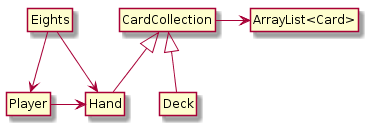
\includegraphics[width=0.75\textwidth]{figs/uml1.png}
\caption{UML diagram for the classes in this chapter.}
\label{fig.uml1}
\end{center}
\end{figure}

Relationships between classes are represented by arrows: composition arrows have a standard arrow head, and inheritance arrows have a hollow triangle head (usually pointing up).
Figure~\ref{fig.uml1} shows the classes defined in this chapter and the relationships among them.

UML is an international standard, so almost any software engineer in the world could look at this diagram and understand our design.
And class diagrams are only one of many graphical representations defined in the UML standard.


\section{Vocabulary}

\begin{description}

\term{inheritance}
The ability to define a new class that has the same instance variables and methods of an existing class.

\term{subclass}
A class that inherits from, or extends, an existing class.

\term{superclass}
An existing class that is extended by another class.

%\term{override}
%To define a method in a subclass that replaces a method with the same name in a superclass.

\term{bottom-up design}
A way of developing programs by identifying simple pieces, implementing them first, and then assembling them into more-complex algorithms.

\term{HAS-A}
A relationship between two classes in which one class ``has'' an instance of another class as one of its attributes.

\term{IS-A}
A relationship between two classes in which one class extends another class; the subclass ``is'' an instance of the superclass.

\end{description}


\section{Exercises}

The code for this chapter is in the {\it ch14} directory of {\it ThinkJavaCode2}.
See page~\pageref{code} for instructions on how to download the repository.
Before you start the exercises, we recommend that you compile and run the examples.


\begin{exercise}  %%V6 Ex14.1

Design a better strategy for the \java{Player.play} method.
For example, if there are multiple cards you can play, and one of them is an 8, you might want to play the 8.

\index{override}

Think of other ways you can minimize penalty points, such as playing the highest-ranking cards first.
Write a new class that extends \java{Player} and overrides \java{play} to implement your strategy.

\end{exercise}


\begin{exercise}  %%V6 Ex14.2

Write a loop that plays the game 100 times and keeps track of how many times each player wins.
If you implemented multiple strategies in the previous exercise, you can play them against each other to evaluate which one works best.

{\em Hint:} Design a \java{Genius} class that extends \java{Player} and overrides the \java{play} method, and then replace one of the players with a \java{Genius} object.

\end{exercise}


\begin{exercise}  %%V6 Ex14.3

One limitation of the program we wrote in this chapter is that it handles only two players.
Modify the \java{Eights} class to create an \java{ArrayList} of players, and modify \java{nextPlayer} to select the next player.

\end{exercise}


\begin{exercise}  %%V6 Ex14.4

When we designed the program for this chapter, we tried to minimize the number of classes.
As a result, we ended up with a few awkward methods.
For example, \java{cardMatches} is a static method in \java{Player}, but it would be more natural if it were an instance method in \java{Card}.

The problem is that \java{Card} is supposed to be useful for any card game, not just Crazy Eights.
You can solve this problem by adding a new class, \java{EightsCard}, that extends \java{Card} and provides a method, \java{match}, that checks whether two cards match according to the rules of Crazy Eights.

At the same time, you could create a new class, \java{EightsHand}, that extends \java{Hand} and provides a method, \java{scoreHand}, that adds up the scores of the cards in the hand.
And while you're at it, you could add a method named \java{scoreCard} to \java{EightsCard}.

Whether or not you actually make these changes, draw a UML class diagram that shows this alternative object hierarchy.

\end{exercise}
